% Set the author and title of the compiled pdf
\hypersetup{
  pdftitle = {\Title},
  pdfauthor = {\Author}
}

\section{Finite precision computation}

Unfortunately, the world is not solely restricted to integers, and computers
often need to work with real numbers $\mathbb{R}$. With integers, the main
problem we have in computer terms is overflow, and since there is a finite
distance from one to the next, they are easy to encode in a computer.

On the other hand, between any two real numbers, there are infinitely many more
real numbers. Since computers are discrete, we need to sample the real numbers
so that we can find a representation for them in the computer. However, this
introduces errors, since we can't represent every value exactly and therefore
most approximate.

\subsection{Floating point numbers}

%Slide 1

One problem we have with computation is that we don't know what the error is
with computations; how `good' is the result of an algorithm or computation? We
would like to know the error bounds of a solution, and have the output be
reliable.

%Slide 2

In the $70$'s, it was realised that different floating point implementations
produced different results. This had significant concerns for reproducability,
and as a result the ANSII IEEE standard for binary floating point arithmetic was
created.

%Slide 3

Each floating point number is represented as four integers; the base, the
precision, the exponent and the mantissa.

\[
  x = \pm m \times b^{e-n}
\]

Where:

\begin{center}
  \begin{tabular}{>{$}l<{$}|l}
    m & The Mantissa (the bit before the decimal place)\\
    b & The base (or radix), usually two or ten\\
    e & The exponent (the power of the radix)\\
    n & The precision (the number of digits in the mantissa)
  \end{tabular}
\end{center}

We can represent different numbers in different ways, for example:

\[
  0.121e10^3 = 0.0121e10^4
\]

In this case, we can normalise the way in which we represent numbers and at
least all computers will get the same errors.

% Slide 4

The amount of numbers we can represent with the floating points depends on the
values permissible for $b,n$ and $e$. When $b=2,n=2$ and $e=[-2\dots2]$:

\marginpar{The Python code used to generate this is found in the
\texttt{/COMP36212/programs} folder of the source for these notes.}

\begin{center}
  \begin{tabular}{>{$}c<{$} >{$}c<{$} >{$}c<{$} >{$}c<{$} >{$}c<{$}}
    2 & \times & 2^{-2} & = & 0.500000\\
    3 & \times & 2^{-2} & = & 0.750000\\
    2 & \times & 2^{-1} & = & 1.000000\\
    3 & \times & 2^{-1} & = & 1.500000\\
    2 & \times & 2^{0} & = & 2.000000\\
    3 & \times & 2^{0} & = & 3.000000\\
    2 & \times & 2^{1} & = & 4.000000\\
    3 & \times & 2^{1} & = & 6.000000\\
    2 & \times & 2^{2} & = & 8.000000\\
    3 & \times & 2^{2} & = & 12.000000\\
  \end{tabular}
\end{center}

The mantissa is always $2$ or $3$ since we're using an explicit one, so the
binary values are either $[1,0]$ or $[1,1]$.

Floating point numbers are relatively spaced; even though they might not be the
same distance apart, the ratio between them is the same. The unit round off
(basically the last digit) is called the \textit{relative machine precision}.

The \textbf{Relative Machine Precision} is given by $u = 0.5 \times b^{1 - n}$,
and is the largest possible difference between a real number and its floating
point representation. In the above example, $u = 0.5 \times 2^{-1} =
\frac{1}{4}$. The value $2u$ is called the \textbf{Machine Precision}.

%Slide 5

In the exam, assume explicit storage of leading bit of mantissa.

\subsubsection{Real world floats}

% TODO: Insert diagram of float format here

For the sign bit, $0$ is for positive numbers and $1$ is for negative ones. The
exponent must also be able to represent negative numbers (in the case of
$24\times2^{-2}$ for example), and thus in single precision floats, a bias of
$+127$ is added to the exponent and that value is stored. The exponent values
$-127$ and $+128$ are reserved for special numbers.

The first bit of the mantissa is implicitly $1$ in the IEEE base two floating
point representation. This is because normalised numbers always have $1$ as the
first digit of their mantissa, and then we can get another digit of precision.

% TODO: Ranges of floating point numbers slide 1

Sixty-four bit floating point numbers have one sign bit, $11$ exponent bits and
$52$ mantissa bits. This means their bias will be $2^11 = 2048$ and the range
will be $2 - 2^{52} \times 2^{2^{11}}$.

The standard also has special values built in:

\begin{description}
  \item \textbf{Zero}: When the exponent is all zeros and the mantissa equal to 
  zero.
  \item \textbf{Denormalised number}: If the exponent is all zero, but the
  mantissa is non-zero, then the number is
  $-1^{sign} \times 0.m\times 2^{-126}$.
  \item \textbf{Infinity}: Exponent is all 1's and mantissa is all 0's. The
  sign dictates between positive and negative infinity.
  %TODO: Signalling and quite NaN's
  \item \textbf{NaN}: Not your grandma, this is when the value isn't a real
  number, such as when a division by zero occurs.The exponent is all 1's and
  the mantissa is non-zero.
\end{description}

\subsubsection{Error in floating point numbers}
% Example exam q:
% Given a decimal number x, convert it to normal form and then into binary
% with specific values for e, m and b. Then trunctuate/round it and estimate
% the error

% TODO: How can a computer work out this error? It only knows floats...

When a real number is converted to floating point number, it may lose precision.
If the real number if $x$ and the floating point representation is
$\bar{x}$, then the error is:

\[
  e = \bar{x} - x
\]

You can find how many significant digits a floating point number approximates a
real number to by doing:

\[
  |\bar{x} - x| = 10^{-\text{significant digits}}
\]


However, the absolute error $e$ does not give us a very good description of the
accuracy (if the error is $10^{-6}$ but the value is $10^{-7}$ then we're very,
very inaccurate)! To rectify this, we have relative error:

\[
  r = \frac{e}{x} = \frac{\bar{x} - x}{x}
\]

%TODO: Wat is bounds?!

When we're getting the floating point number from the real number, we can
truncate the (possibly infinite) digits so that it fits in the mantissa. Simply
chopping the number so it fits in $m$ bits is called \textbf{simple truncation}.

If we round numbers instead of using simple truncation, then we can reduce the
error. We need some rules though:

\begin{itemize}
  \item If the part of the mantissa to be chopped of is less than $0.5$, use
  simple truncation.
  \item If it's greater, then increment the last digit of the mantissa, and then
  truncate.
  \item If it's equal to $0.5$, then we can do either (though IEEE says to round
  up).
\end{itemize}

Now the relative error is:

\[
  |r| = \frac{|e|}{|x|} = \frac{0.5 \times b^{e-n}}{|m|\times b}
      = \frac{1}{2 \times m \times b^n}
\]

There are three types of errors that computers can make:

\begin{itemize}
  \item Essential errors are ones that cannot be avoided (e.g. from erroneous
  input).
  \item Rounding errors are when we have to approximate real numbers with
  floating point ones. This error can be measured and controlled.
  \item Methodology errors come into play when replacing one problem by another
  similar, easier but less accurate problem is done. The solution is close, but
  not exact.
\end{itemize}

Unfortunately, errors can propagate through a computation. We must know the
errors introduced by every operation a computer performs on floating point
numbers. If we know $e_x = \bar{x} - x$ and $e_y = \bar{y} - y$, what is $e_{x
\cdot y}$?

The error introduced by addition, subtraction, multiplication and division is:

\begin{description}
  \item Addition:
  \[
    \bar{x} + \bar{y} = (x + e_x) + (y + e_y) = (e_x + e_y) + (x + y)
  \]
  \[
    e_{x+y} = e_x + e_y
  \]
  \item Subtraction:
  \[
    e_{x-y} = e_x - e_y
  \]
  \item Multiplication:
  \[
    \bar{x} \times \bar{y} = (x + e_x) \times (y + e_y) =
      xy + xe_y + ye_x + e_xe_y
  \]
  \[
    e_{x \times y} \approx xe_y + ye_x
  \]
  \item Division:
  %TODO: Equation here...
  \[
    e_\frac{x}{y} \approx \frac{1}{y}e_x - \frac{x}{y^2}e_y
  \]
\end{description}

Relative error can also be calculated:

\begin{description}
  \item Addition:
    \[
      r_{x+y} = \frac{e_{x+y}}{x + y} = \frac{x}{x + y}r_x + \frac{y}{x + y}r_y
    \]
  \item Subtraction:
    \[
      r_{x-y} = \frac{e_{x-y}}{x - y} = \frac{x}{x - y}r_x + \frac{y}{x - y}r_y
    \]
  \item Multiplication:
    \[
      r_{x \times y} = \frac{e_{x \times y}}{x \times y} \approx r_x + r_y
    \]
  \item Division:
    \[
      r_{x / y} = \frac{e_{x / y}}{x / y} \approx r_x - r_y
    \]
\end{description}

In general, $\bar{x} \circ \bar{y} = (x \circ y)(1 + r_{x \circ y})$.

\marginpar{Remember, error propagation is not associative. The error from a
multiplication and then an add is probably not the same as doing the add then
the multiplication.}

While it is useful to know the error of one operation, we also need to be able
to work out the error of consecutive operations. That is to say given $e_x =
\bar{x} - x$ and  $e_y = \bar{y} - y$, determine $e_{x \bar{\circ} y}$.
\[
  \begin{split}
  \bar{x} &= FP(\bar{x_1} \circ \bar{x_2})\\
          &= \bar{x_1} \bar{\circ} \bar{x_2}\\
          &= (\bar{x_1} \circ \bar{x_2})(1 + u)\\
  \end{split}
\]

Where $|u| \leq 0.5 \times b^{-n + 1}$.

The total relative error is given by:

\[
  r^t_z = \frac{e^t_z}{x} = r_{x \circ y} + u = a_xr_x + a_yr_y + u
\]

$a_x$ and $a_y$ is the error introduced by the $\circ$ operation.

Lets put all that into an example. Given the numbers $x,y$ and $x$ with their
relative round off errors $r_x, r_y$ and $r_z$, determine the relative error in
$u = (x + y)z$:

\[
  r^t_{x + y} = \frac{x}{x + y}r_x + \frac{y}{x + y}r_y + r_+
\]

%TODO: Ask Milan about this slide (23)

\[
  r^t_{u} = \frac{x}{x + y}r_x + \frac{y}{x + y}r_y + r_+ + r_z + r_*
\]

We can work out the unit round off errors somehow...

%END TODO


\subsection{Finding the number of significant digits}

We want to find an integer that represents how many digits in our number are
non-nonsense (i.e. how many significant digits we have). The number of
significant digits in the floating point number $\bar{x}$ where its real
equivalent is $x$ is:

\marginpar{Z is the set of integers.}

\[
  l = Z(log_b\frac{|x|}{|\bar{x} - x|})
\]

If we rearrange this, the relative error is:

\[
  r_x \approx b^{-l}
\]

If we have a computation that takes $m$ real numbers as arguments and outputs a
real number, if the arguments are floating point numbers with $l_i$ significant
digits then we can estimate:

\[
  |e| \approx |\sum^m_{i=1} x_i\frac{\delta f}{\delta x_i}b^{-l_i}|
\]

Also:

\[
  |\sum^m_{i=1} x_i\frac{\delta f}{\delta x_i}b^{-l_i}|
    \leq b^{-l_{min}}|\sum^m_{i=1} x_i\frac{\delta f}{\delta x_i}|
\]

The number of significant digits in the answer is:

\[
  l = l_{min} - \delta
\]

Where $\delta$ is the loss of significant digits:

\[
  \delta = Z(log_b(
    \frac{
      \sum^m_{i=1}|x_i\frac{\delta f}{\delta x_i}|
    }{
      |f(x_1, \dots, x_m)|
    }
  )
\]

If we try and subtract numbers that are close in magnitude, then we will lose
lots of significant digits. If we do $\sqrt{2.01} - \sqrt{2}$ (where both
numbers are known to 9 significant digits), then we get:

\[
  \delta = Z(log_10(
    \frac{
      |\sqrt{2.01}| + |\sqrt{2}|
    }{
      |\sqrt{2.01} - \sqrt{2}|
    })) = 3
\]

Our answer would be to six significant figures. In order to get all of the
significant figures, we need to use a different method:

\[
  \begin{split}
    z &= \sqrt{2.01} - \sqrt{2}\\
      &= (\sqrt{2.01} - \sqrt{2})\frac{\sqrt{2.01}
         + \sqrt{2}}{\sqrt{2.01} + \sqrt{2}}\\
      &= \frac{\sqrt{2.01}^2 - \sqrt{2}^2}{\sqrt{2.01} + \sqrt{2}}\\
      &= \frac{0.01}{\sqrt{2.01} + \sqrt{2}}
  \end{split}
\]

\marginpar{Revision break? Read this:
\href{https://randomascii.wordpress.com/2014/01/27/theres-only-four-billion-floatsso-test-them-all/}{https://randomascii.wordpress.com
/2014/01/27/theres-only-four
-billion-floatsso-test-them-all/}}

\subsubsection{Accurately computing sample variance}

Computing the sample variance of a set of numbers is done by the formula:

\[
  s^2_n = \frac{1}{n - 1}\sum^n_{i=1}(x_i - \hat{x})^2
\]

Where $\hat{x} = \frac{1}{n}\sum^n_{i=1}x_i$ is the mean of the values.

In order to compute the variance, we would need to calculate the mean first,
then calculate the variance, which requires two for loops. However, a
numerically equivalent formula exists for doing the same thing:

\[
  s^2_n = \frac{1}{n-1}(\sum^n_{i=1}x_i^2 - \frac{1}{n}(\sum^n_{i=1}x_i)^2)
\]

If we use the following data:

\begin{center}
  \begin{tabular}{>{$}c<{$}|>{$}c<{$}}
    \text{Value} & \text{Floating point representation}\\ \hline
    100 & 0.1000\times10^3\\
    101 & 0.1010\times10^3\\
    102 & 0.1020\times10^3
  \end{tabular}
\end{center}

If we use formula one for the variance with these input numbers, then we get an answer of $1$, if we use formula two, then we get the answer to be $-1.667$

% TODO: Why???

\subsubsection{Overflow and underflow}

We must be aware of overflow and underflow in our operations. For example, if we
were calculating the length of the hypotenuse of a triangle
($\sqrt{\text{opposite}^2 + \text{adjacent}^2}$), then we could have an overflow
if $x = y = 10^{200}$, since the range representable by a single precision float
is $10^{\pm308}$.

This can be remedied by using a different formula:

\begin{center}
  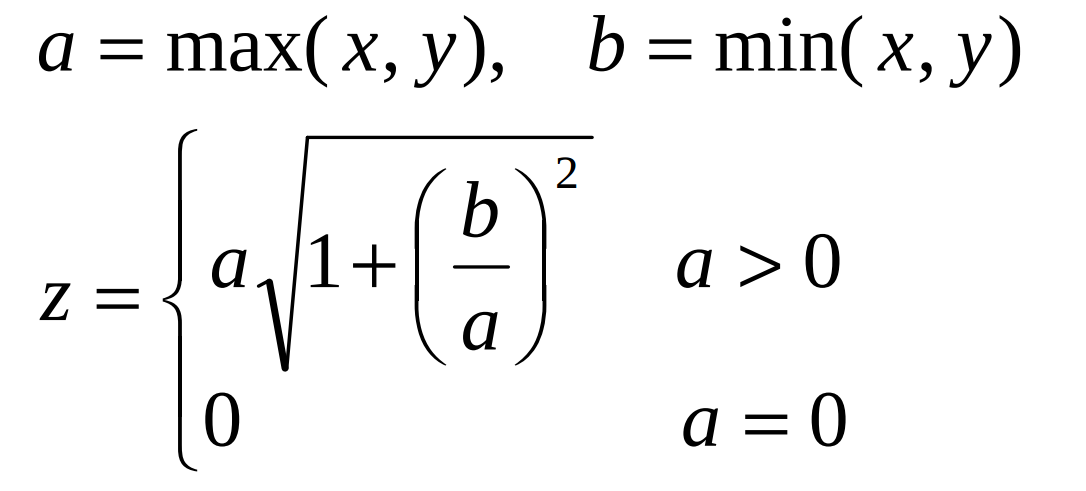
\includegraphics[width=0.3\textwidth]{images/safe-pythag}
\end{center}

\subsection{Condition of a problem}

The condition of a problem is how sensitive it is to changes in the data. A
problem is ill-conditioned if a small change in the data results in a large
change in the solution. This is concerned with the problem, not the method used
to solve it.

Consider the equation $x^3 - 21 x^2 + 120x - 100 = 0$; the solutions are $x =
\{1, 10\}$. However, if we change the value of $x^3$ to $0.99$ or $1.01$, then
the roots become $x = \{1, 11.17, 9.041\}$ and $x = \{1, 9.896 \pm 1.044\}$
respectively.

We can work out the sensitivity by using partial differentiation, if the
perturbed function if $\bar{f}(x) = f(x) + \epsilon g(x)$, where $g(x)$ is the
change applied to $f(x)$, then:

\[
  |\delta| \approx |\frac{\epsilon g(x)}{f'(x)}|~\text{(single root)}
\]

\[
  |\delta| \approx |\sqrt{-\frac{2\epsilon g(x)}{f''(x)}}|~\text{(double root)}
\]

In the above example, $g(x) = x^3, \epsilon = -0.01, f'(x) = 3x^2 - 42x + 120$:

\[
  |\delta| \approx |\frac{-0.01 \times 1^3}{81}| \approx 0.0001
\]

For the double root, $f''(x) = 6x - 42$

\[
  |\delta| \approx |\sqrt{-\frac{2 \times -0.01 \times 1000}{18}}| \approx 1.054
\]

So the double root is vastly affected, but the single root isn't.

\subsection{Stability}

The stability of a method is how sensitive it is to rounding errors. A method
that guarantees as accurate solution as the input data allows is said to be
stable, otherwise it's unstable. Condition is about the sensitivity of the
problem, but stability is about the sensitivity of the method.

Given the quadratic equation $1.6x^2 - 100.1x + 1.251 = 0$, the solution can be
found using the standard formula (in floating point) ($x = \frac{-b \pm\sqrt{b^2
- 4ac}}{2a}$), which gives $x = \{62.53, 0.03125\}$.

If we only compute the first root to be $x_1 = 62.53$, but use $x = c/ax_1$ for
the second, then we get the second root to be $0.01251$. The correct solutions
are $x = \{62.53, 0.0125\}$.

The problem was that $y_1 = -b = 100.1$, and  $y_2 = \sqrt{b^2 - 4ac} = 100.06$.
Since if we do subtraction with very close numbers, the error is high. If we
calculate $\delta$ for this then we get:

\[
  \delta = X(log_10\frac{|y_1| + |y_2|}{|y_1 - y_2|}) = 4
\]

Meaning all of our digits were rubbish!

%TODO: Page 41 onwards for an example

% Part two of the course!

\section{Optimisation and nature inspired algorithms}

To start, lets recap some stuff you should already know; a minima is a point of
a function where all points in its vicinity have a higher value than itself,and
a maxima is the opposite; a point where all points in its vicinity have a lower
value than itself.

Since we can invert a function by putting a minus in front of it, we don't
really need to differentiate between maxima and minima, since we can always
express on in terms of the other.

Global optimums are the best values for the entire domain, while local optimums
are best in some bounded region.

One dimensional functions are easiest to visualise; they are just a graph, where
the y value is the value of the function and the x value is the input. As the
dimensionality increases, the functions get harder to visualise; 2d functions
are visualised on a 2d graph, where the intensity of the colour in each square
represents the value of the function at that coordinate. 

% TODO: inequality/equality constraints?

An optimisation problem is one where we attempt to maximise or minimise a
function. This involves finding the input that will produce the largest or
smallest value. Optimisation problems are really search problems; given a
domain, find an input that produces the smallest output.

If we know exactly what the function we're trying to optimise is (i.e. we have
an equation), then it's an explicit problem, but if we just have some inputs and
outputs, then it's a black box problem.

Similarly, there are two different approaches to solving these problems:

\begin{description}
  \item \textbf{Single solution}:\\
   This is where there is a single candidate solution that is incrementally 
   improved by the algorithm throughout the procedure.
  \item \textbf{Population based solution}:\\
    This is where there is a set of candidate solutions (the population) and an
    iterative operation combines the best ones to improve the quality of the 
    population.
\end{description}

All of the optimisation methods follow a cycle:

\begin{itemize}
  \item Guess some parameters for the initial solution
  \item While we're not satisfied:
  \begin{itemize}
    \item Evaluate how the current parameters perform
    \item If we're satisfied, then we've finished
    \item Otherwise, then determine new parameters based on the current ones
      and their evaluation.
  \end{itemize}
\end{itemize}

We can use derivatives to try and find maxima and minima in a function. If we do
not have an explicit function for the derivative, then we can calculate them
using \textbf{finite differences}:

\begin{description}
  \item \textit{Forward difference}:\\
    \[
      f'(x) \approx \frac{f(x + h) - f(x)}{h}
    \]
  \item \textit{Central difference}:\\
    \[
      f'(x) \approx \frac{f(x + h) - f(x - h)}{2h}
    \]
\end{description}

Here, the $h$ parameter is the range over which we're calculating the
differential.

\subsection{Minimising univariate functions}

For one dimensional functions, we can use two approaches:

\begin{itemize}
  \item Interval reduction, where we iteratively reduce the range of values that
  we think the optimum is inside.
  \item Interpolation, where we try to find an approximate function and use the
  optimum of that function to iterate to find a better approximate function.
\end{itemize}

\subsubsection{Bisection algorithm}

This is the easiest algorithm, we start with the full range in the domain, and
then cut it in half based on the value of the differential at the midpoint at
the range.

\begin{verbatim}
  bisection(f'(x), a, b, e) {
    while (b - a >= e) {
      c = (a + b) / 2;
      if (f'(c) < 0) a = c;
      else if(f'(c) > 0) b = c
      else return c;
    }
  }
\end{verbatim}

\subsubsection{Quadratic interpolation algorithm}

Here, we make a quadratic function that goes through three points $a, b$ and
$c$, then we either drop $a$ or $b$ depending on which way we should move the
quadratic function. Here, \textbf{we do not need the differential} which is good
since we won't always have it!

% TODO: Insert & explain psudo code

\begin{verbatim}
  Sudo insert psudo code
\end{verbatim}

\subsubsection{Stopping criteria}

Eventually, we will have to stop our optimisation algorithms, but some of them
will run indefinitely. We need criteria to make them stop after a sane amount of
time. The simple approach is to stop after $n$ iterations, and is applicable to
all iterative functions. The more clever approach is to only stop when we reach
a certain threshold, i.e. when a method converges asymptotically on an optimum.
